\documentclass[border=4pt]{standalone}
\usepackage{tikz}
\usetikzlibrary{arrows,positioning}
\begin{document}
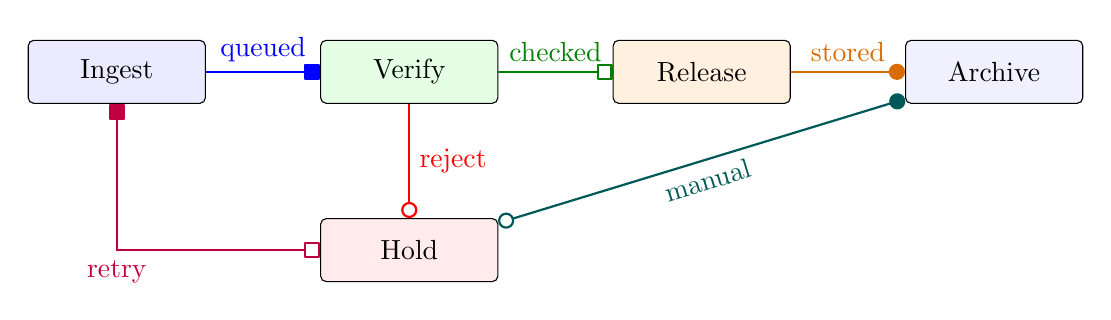
\begin{tikzpicture}[
  node distance=1.45cm,
  stage/.style={draw,rounded corners=2pt,minimum width=2.25cm,minimum height=8mm,align=center}
]
  \node[stage,fill=blue!8] (ingest) {Ingest};
  \node[stage,fill=green!10,right=of ingest] (verify) {Verify};
  \node[stage,fill=orange!12,right=of verify] (release) {Release};
  \node[stage,fill=blue!6,right=of release] (archive) {Archive};
  \node[stage,fill=red!8,below=of verify] (hold) {Hold};

  \draw[blue,line width=.8pt,-square] (ingest) -- node[above]{queued} (verify);
  \draw[green!50!black,line width=.8pt,-{open square}] (verify) -- node[above]{checked} (release);
  \draw[orange!85!black,line width=.8pt,-*] (release) -- node[above]{stored} (archive);
  \draw[red,line width=.8pt,-o] (verify) -- node[right]{reject} (hold);
  \draw[purple,line width=.8pt,{open square}-{square}] (hold) -| node[below]{retry} (ingest);
  \draw[teal!70!black,line width=.8pt,{o}-{*}] (hold) -- node[below,sloped]{manual} (archive);
\end{tikzpicture}
\end{document}
